\documentclass[a4paper,12pt,titlepage]{article}

\usepackage[utf8]{inputenc}
\usepackage[T1]{fontenc}
\usepackage[french]{babel}
\usepackage{color}
\usepackage[hmargin={2.5cm,2.5cm},top=2.5cm,bottom=2.5cm]{geometry}
\usepackage{graphicx}
\usepackage[colorlinks=true,breaklinks=true,linkcolor=blue,filecolor=magenta,urlcolor=cyan,pdftitle={Rapport AP4A},pdfsubject={Rapport AP4A}]{hyperref}
\usepackage{listings}
\usepackage{tikz, pgf}
\usepackage[ruled,lined]{algorithm2e}
\usepackage{calc}

\newenvironment{alandscape}
{
    \newpage
    \pdfpagewidth=\dimexpr 2\pdfpagewidth\relax
    \setlength{\textwidth}{\dimexpr 4cm + 2\textwidth\relax}
    \headwidth=\textwidth
    \hsize=\textwidth
}
{
    \newpage
    \pdfpagewidth=\dimexpr .5\pdfpagewidth\relax
    \setlength{\textwidth}{\dimexpr \textwidth - 4cm\relax}
    \textwidth=\dimexpr .5\textwidth\relax
    \headwidth=\textwidth
    \hsize=\textwidth
}


\title{Rapport AP4A}
\author{Corentin \bsc{HAUTEFAYE}}
\date{Novembre 2025}

\begin{document}

\SetKwComment{Comment}{/* }{ */}
\SetKwInput{Entree}{Entrée}
\SetKwInput{Sortie}{Sortie}
\SetKw{KwA}{à}
\SetKw{KwD}{de}
\SetKw{KwO}{OU}
\SetKw{KwE}{ET}
\SetKw{KwN}{NON}
\SetKwBlock{Deb}{Début}{Fin}
\SetKwIF{Si}{SinonSi}{Sinon}{Si}{Alors}{Sinon\:si}{Sinon}{Fin\:Si}
\SetKwFor{Pour}{Pour}{Faire}{Fin\:Pour}
\SetKwFor{Tq}{Tant que}{Faire}{Fin\:Tant\:que}
\SetKwRepeat{Rep}{Répéter}{Jusqu'à}
\SetKwProg{Fn}{Fonction}{\\Début}{Fin}
\SetKwProg{Pc}{Procédure}{\\Début}{Fin}

\SetAlgorithmName{Algorithme}{}{}

\maketitle

\renewcommand{\abstractname}{Introduction}
\begin{abstract}
    Dans le cadre de l'UE AP4A (\textit{Semestre A25}), nous avons réalisé un mini-projet qui a pour but de simuler et modéliser des interactions entre badges d'accès et lecteurs associés. En somme, l'objectif est de mettre en œuvre les techniques élémentaires de la programmation orientée objet C++, pour ici le contrôle sécurisé des accès à des bâtiments, ou des salles quelconques sur par exemple un campus d'université, ou au sein d'une entreprise.
\end{abstract}
%-----------------------------------------------
\tableofcontents
\newpage
%-----------------------------------------------
\section{Présentation}
\subsection{Définition du sujet}
On modélise un système de badges par un serveur communiquant avec les badges et lecteurs de badges pour déterminer si une requête d'accès donnée est recevable ou non. Bien entendu afin de simplifier notre modèle, on ne considère un vrai serveur, mais plutôt les liens et interactions entre les objets. De ce fait, on définit un acteur supplémentaire, que l'on appellera ici l'ordonnanceur, qui permettra d'initier diverses requêtes au serveur à intervalle de temps régulier.

Notons en sus de cela qu'à chaque badge et lecteur de badge, un niveau de sécurité est associé. Ainsi, si un individu dispose d'un niveau inférieur à celui requit par la porte, la requête est réfutée. Il est également demandé de consigner les demandes fructueuses ou non dans respectivement deux fichiers de journalisation.
\subsection{Conventions}
Afin de répondre au sujet et de le rendre le plus complet possible, de nombreux choix ont été effectués. Tout d'abord, notons que pour une bonne organisation et cohérence dans les fichiers et noms de classe, d'attributs, ..., il a été décidé de tout écrire en Anglais. En effet, cela offre une meilleure lisibilité, notamment quand on cherche à se documenter sur un nouveau projet.

Ensuite, en terme de typographie, afin de rester conforme à la norme, il a été convenable d'utiliser le "camelCaseStyle". Pour rappel, ce dernier consiste à nommer ses variables en attachant tous les mots qui, hormis pour le premier, prennent tous une majuscule. De plus, les pratiques suivantes ont également été mises en œuvre :
\begin{itemize}
    \item Les classes commencent toujours par une majuscule.
    \item Les enumérateurs sont en majuscules.
    \item Les interfaces, à l'instar de Java, juxtapose le préfixe "I" au nom de classe courante.
    \item Le code C++ des classes est séparé de l'entête, sauf pour certains cas triviaux.
    \item Enfin, les fichiers ne contenant pas de classe prennent une minuscule en début de nom.
\end{itemize}

\subsection{Outils utilisés}
Pour réaliser ce projet, les outils suivants ont été utilisés:
\begin{itemize}
    \item \textbf{GCC} pour la compilation
    \item \textbf{CLion} pour l'environnement de développement 
    \item \textbf{Git} et \textbf{GitHub} pour le contrôle des versions
    \item \textbf{clang-uml} pour une première génération du diagramme UML
    \item \textbf{\LaTeX} et \textbf{Overleaf} pour la rédaction du rapport
\end{itemize}

Il est enfin important de rappeler que le projet a été réalisé avec la norme C++17. De plus, les pointeurs intelligents \verb|std::shared_ptr<T>| ont été utilisés afin de pouvoir utiliser le polymorphisme dans le meilleur cas possible.
%-----------------------------------------------
\section{Conception}
\subsection{Architecture}
Dans cette partie sont présentées succinctement les classes et sous-classes principales du projet. Les choix effectués y sont également décrits.

\subsubsection{Espace de noms "badge"}
Afin de simplifier l'implémentation, j'ai choisi de définir un espace de noms dans le fichier \verb|const.h| dans lequel des enumérateurs (constantes) sont présentes. On peut noter notamment les constantes des niveaux de sécurité ainsi que des codes d'erreurs dans le cas où une requête d'appareillage échoue. Bien qu'il soit possible d'utiliser un fichier externe afin d'importer ces paramètres, j'ai trouvé cela superflu dans la mesure où ce n'est qu'un problème secondaire. Toutefois, remarquons que la généricité de l'architecture permet une telle fonctionnalité.

\subsubsection{Ordonnanceur}
La classe \verb|Scheduler| se charge de garder les serveurs en mémoire, et d'initier des requêtes pour un serveur donné. De ce fait, elle a trois attributs :
\begin{itemize}
    \item \verb|servers| qui est un vecteur de pointeurs partagés sur des serveurs. Une telle mise en œuvre permet de gérer plusieurs serveurs, par exemple dans le cas d'une université, plusieurs campus. Un serveur n'a pas accès aux badges et lecteurs d'un autre serveur.
    \item \verb|numSimulations| dans le constructeur, qui permet de définir combien de cycles l'ordonnanceur doit exécuter avant de se mettre en veille.
    \item \verb|sleepTime| qui définit le temps en millisecondes pendant lequel l'ordonnanceur attend avant de passer au prochain cycle.
\end{itemize}

Il contient la méthode \verb|simulate| qui pour un serveur donné, prend aléatoirement un badge et un lecteur et essaie de le appareiller. Celle-ci est détaillée en section \ref{l_sim}. L'ordonnanceur se charge également de créer au démarrage les serveurs présents à partir du fichier \verb|servers.txt|. 

\subsubsection{Serveur}
La classe \verb|Server| modélise, comme son nom l'indique, un serveur. On attribue un nom unique à chaque qui permet de l'identifier. Il dispose des champs \verb|badges| et \verb|readers| qui stockent dans une table de hachage respectivement les badges et lecteurs associés à ce serveur, et leurs identifiants comme clefs. Le serveur peut également accéder au propriétaire du badge en utilisant la méthode appropriée de ce dernier. Il peut être activé ou désactivé à l'aide des méthodes membres correspondantes. Enfin, cet objet supporte le flux de redirection \verb|<<|, utilisé notamment après avoir acquitté une demande d'accès. D'où la présence des attributs \verb|bufferId[2]| qui stocke dans cet ordre les identifiants du badge et du lecteur de la dernière requête ou -1 quand elle a été acquittée, et \verb|errorId| qui stocke le code d'erreur d'une requête qui a échoué et 0 sinon.
\subsubsection{Badge}
Un badge doit être capable au minimum d'être relié à une personne, qui dispose elle-même d'un droit d'habilitation. Il doit également avoir un identifiant unique. Aussi, j'ai trouvé intéressant de faire en sorte, à l'instar des cartes UTBM, d'avoir une date d'expiration, ainsi qu'une liste de droits d'accès à des salles données. Par exemple, certains groupes de GMC, bien qu'ils ne soient qu'étudiants, ont accès à l'aide de leur carte à des salles de travaux pratiques dédiées.

\paragraph{IBadge} On met en place un "contrat" à l'aide d'une interface qui permet de définir ce que fait un badge, sans savoir comment il le fait. Ainsi, il définit les points explicités ci-dessus.

\paragraph{Badge} Il s'agit de l'implémentation triviale d'un badge qui suit le modèle imposé par son interface.

\subsubsection{Personne}
Cet objet permet de définir une personne par son nom et son niveau d'habilitation. La structure actuelle permet des duplicatas de noms, comme dans la vraie vie, dans la mesure où les identifiants des badges dans le serveur sont uniques.

\paragraph{IPerson} La classe abstraite qui reprend les points au-dessus.

\paragraph{Person} Une implémentation triviale respectant son interface. Notons qu'une instanciation de cette classe dispose du niveau de sécurité -1, réfuté par tous les lecteurs. Cela est faux cependant si le badge associé dispose de permissions supplémentaires.

\paragraph{Student} Issue de la classe \verb|Person|. Dispose d'un niveau 0.
\paragraph{Teacher} Issue de la classe \verb|Person|. Dispose d'un niveau 1.
\paragraph{Doctor} Issue de la classe \verb|Person|. Dispose d'un niveau 2.
\paragraph{CleanupStaff} Issue de la classe \verb|Person|. Dispose d'un niveau 3.
\paragraph{Staff} Issue de la classe \verb|Person|. Dispose d'un niveau 4.

\subsubsection{Lecteur}
Le lecteur suit une approche similaire à \verb|IPerson| pour la gestion des niveaux de sécurité. Il doit être capable d'avoir un identifiant unique et un nom, qui supporte les duplicatas. En effet, il est possible d'avoir deux accès différents pour une même salle. Toutefois, pour des soucis de lecture, il est préférable de donner deux noms différents aux lecteurs dans ce cas. Ensuite, il est possible d'activer ou de désactiver un lecteur. Enfin, il doit être capable de connaître une plage horaire d'activation. Par exemple, si la plage est de 07h00 à 21h00, une requête à 21h01 sera refusée. 

\paragraph{IReader} La classe abstraite qui reprend les points au-dessus.

\paragraph{Reader} Une implémentation qui respecte le contrat de l'interface.

\paragraph{RoomReader} Issue de la classe \verb|Reader|. Autorise les individus avec un niveau d'au moins 0 à entrer.

\paragraph{TeacherReader} Issue de la classe \verb|Reader|. Autorise les individus avec un niveau d'au moins 1 à entrer.

\paragraph{LabReader} Issue de la classe \verb|Reader|. Autorise les individus avec un niveau d'au moins 2 à entrer.

\paragraph{CleanupReader} Issue de la classe \verb|Reader|. Autorise les individus avec un niveau d'au moins 3 à entrer.

\paragraph{StaffReader} Issue de la classe \verb|Reader|. Autorise les individus avec un niveau d'au moins 4 à entrer.

\subsection{Algorithmes clefs}
\subsubsection{Traiter une requête}
Le serveur se charge de traiter une demande d'accès à l'aide des identifiants du badge et du lecteur avec lequel on souhaite s'appareiller, d'où la méthode \verb|queryAccess|. Pour cela, on doit appliquer les tests suivants:
\begin{enumerate}
    \item Vérifier que le badge et le lecteur existent pour les identifiants donnés.
    \item Vérifier si le lecteur est activé.
    \item S'assurer que le badge n'a pas expiré (i.e date actuelle inférieure à celle de la carte).
    \item \begin{itemize}
        \item S'assurer que le badge dispose d'un niveau de sécurité d'au moins celui du lecteur.
        \item Sinon, vérifier si l'identifiant du lecteur fait partie des permissions accordées au badge.
    \end{itemize}
    \item Vérifier que l'on fait la demande d'accès pendant l'intervalle de fonctionnement du lecteur (cf. \ref{l_plage}).
\end{enumerate}

Si un des tests précédents échoue, la méthode renvoie faux et met à jour le champ \verb|errorId| du serveur. Notons que les identifiants sont également sauvegardés dans le buffer \verb|bufferId[2]|.

\subsubsection{Simuler des requêtes} \label{l_sim}
L'ordonnanceur se charge de simuler les requêtes, notamment à l'aide de la méthode éponyme \verb|simulate|. 
\begin{enumerate}
    \item On choisit un identifiant aléatoire dans les clefs des tables de hachage du serveur, d'où un badge et un lecteur.
    \item On appelle ensuite la méthode \verb|queryAccess| avec ces derniers, puis selon la réussite ou non de la demande, on redirige la sortie du serveur vers le journal approprié, puis vers la console.
    \item Enfin, on nettoie les drapeaux d'erreur du serveur.
\end{enumerate}

\subsection{Gestion du temps}
La gestion de la date et du temps est toujours un problème compliqué en Informatique. Ici, l'utilisation de la norme C++17 ne permet pas d'utiliser les mécanismes modernes d'horloge de la bibliothèque \verb|<chrono>|. Par conséquent, j'ai choisi de définir quelques fonctions afin de gérer les opérations sur des temps, ainsi que le type \\\verb|std::chrono::system_clock::time_point|.

\label{l_plage} Il a été également nécessaire de définir la classe \verb|TimeSlot| qui représente un intervalle de temps. Il est à noter que comme \verb|<chrono>| se base sur le temps de la machine, la partie qui vérifie si on fait une requête au bon moment de la journée est désactivée. En effet, si le projet est corrigé à un moment où tous les lecteurs ne sont pas actifs, aucune demande ne pourrait aboutir. Le code est néanmoins toujours présent dans la méthode \verb|queryAccess|, bien que commenté.

\subsection{Gestion des fichiers}
\subsubsection{Configuration}
Les fichiers présentés doivent être placés dans le dossier où se trouve l'exécutable. Des fichiers exemples sont présents à la racine du fichier ZIP.

\paragraph{servers.txt} Chaque ligne de ce fichier contient le nom d'un serveur. Ce dernier doit être unique et ne peut pas contenir de caractères non-ASCII, sous peine de provoquer des comportements indésirables ou inopinés.

\paragraph{s\_[nom du serveur].txt} Ce fichier est composé de deux parties, séparées par une ligne avec un unique point virgule. Il contient les informations de badges, personnes et lecteurs.
Dans un premier temps, chaque ligne représente une personne et un badge. Elle est de la forme suivante (les sauts de ligne sont uniquement présents pour une bonne lecture):

\begin{verbatim}
    [Nom];[Niveau de sécurité (de 0 à 4)];
\end{verbatim}

\begin{verbatim}
    [Identifiant unique (entier naturel)];[YYYY-MM-DD HH:MM];
\end{verbatim}

\begin{verbatim}
    [Liste des lecteurs autorisés (facultatifs, éléments séparés par ;)]
\end{verbatim}

Dans un second temps, les informations sur les lecteurs sont chargés, ligne par ligne. Elles sont de la forme suivante:

\begin{verbatim}
    [Nom];[Niveau de sécurité];
\end{verbatim}

\begin{verbatim}
    [Identifiant unique];[0 ou 1 si activé];
\end{verbatim}

\begin{verbatim}
    [YYYY-MM-DD HH:MM (début plage)];[YYYY-MM-DD HH:MM (fin plage)]
\end{verbatim}

Il est à noter que la partie date de la plage du lecteur n'est pas utile pour les tests. De plus, ce fichier ne doit pas terminer sur une ligne vide.

\subsubsection{Journaux}

\paragraph{log\_s\_[nom du serveur].log} Ce fichier contient toutes les demandes d'accès ayant été autorisées.

\paragraph{log\_f\_[nom du serveur].log} Ce fichier contient toutes les demandes d'accès qui ont échoué.

\subsection{Diagramme de classes UML}
Un fichier \verb|uml.png|, bien plus lisible, est disponible dans le dossier docs.

\begin{alandscape}
    \begin{figure}[H] 
        \centering
        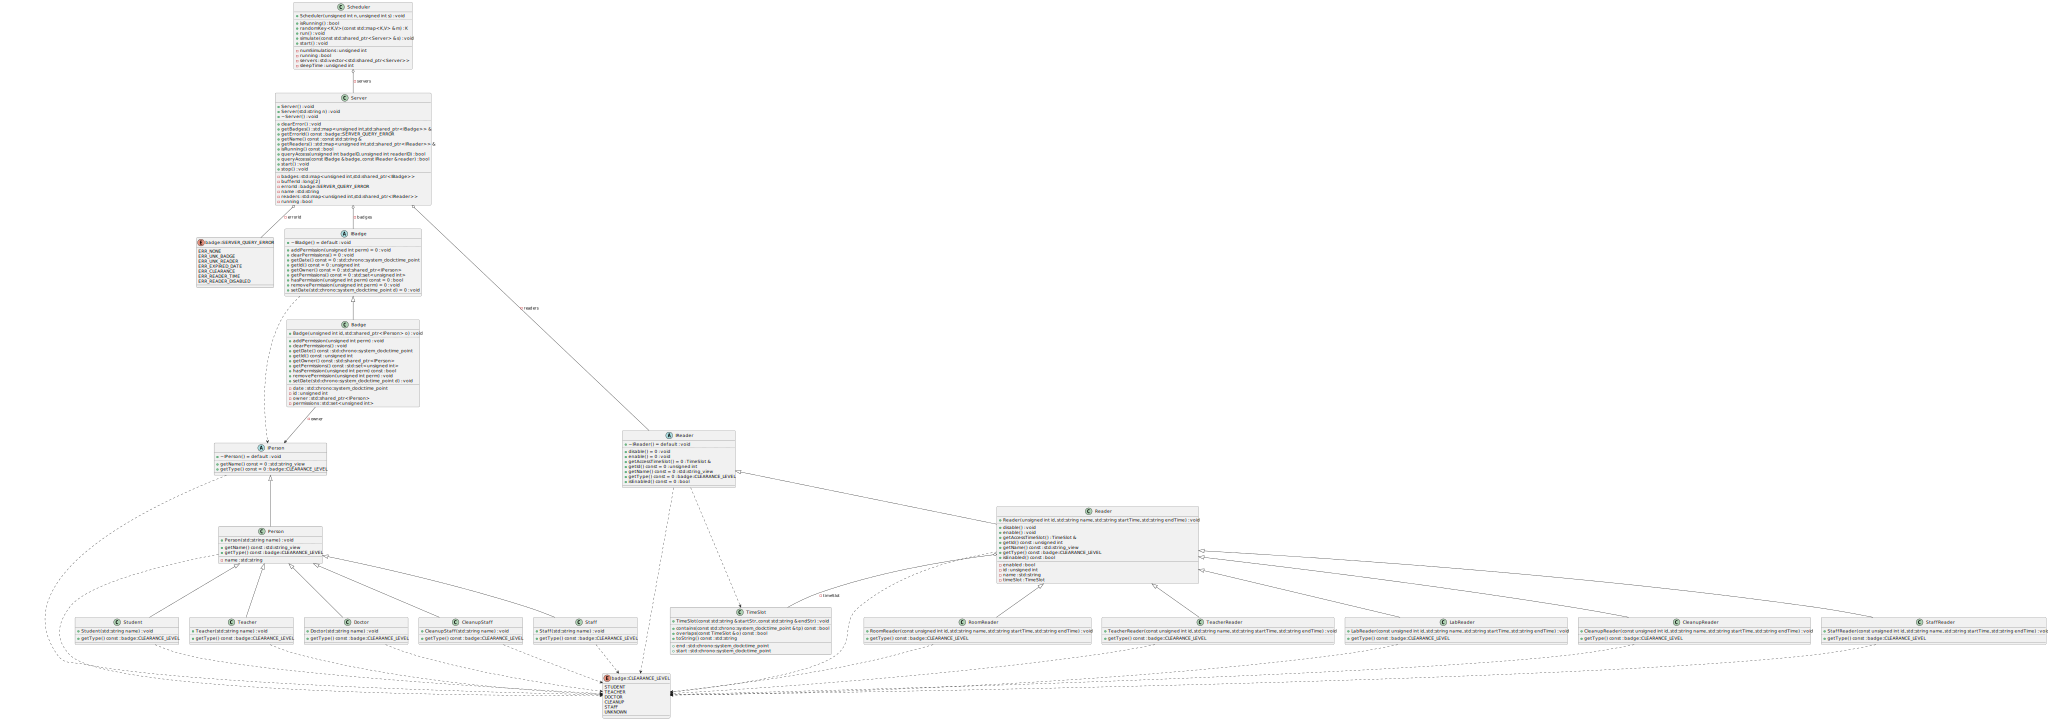
\includegraphics[width=3.0\linewidth]{uml.png}
    \end{figure}
\end{alandscape}

%-----------------------------------------------
\newpage
\section{Retour d'expérience}
\subsection{Difficultés rencontrées}
Les seules difficultés que j'ai rencontrées sont liées à l'utilisation des pointeurs intelligents, car bien que je connaissais leur existence, je n'y avais jamais touché auparavant. Toutefois, cela a constitué une expérience intéressante et enrichissante sur ce point.

Il est vrai aussi que j'ai eu parfois du mal à cibler exactement ce qui était attendu. J'ai en effet trouver que les consignes étaient assez vagues par moments, d'où les choix que j'ai dû entreprendre.

Enfin, la réalisation et la mise en page du diagramme des classes UML dans ce rapport n'a pas été triviale, surtout la mise en page.

\subsection{Suggestions d'amélioration}
Il y a bien des points où mon projet pourrait être amélioré. J'ai tout d'abord conscience du fait qu'il n'est pas entièrement optimisé. Néanmoins, pour les points concernés, il s'agit de choses souvent minimes.

Ensuite, il pourrait être intéressant d'utiliser une vraie base de données, ou dans le pire des cas, un fichier JSON pour la configuration et le stockage des données sur le serveur.

Enfin, les droits d'accès définis dans \verb|const.h| pourraient être chargés depuis un fichier.
%-----------------------------------------------
\newpage
\section{Conclusion}
Ce mini-projet m’a permis de consolider mes compétences en programmation orientée objet en C++. À travers la conception d’un simulateur de contrôle d’accès, j’ai pu explorer des notions clefs telles que l’héritage, le polymorphisme, la gestion des fichiers et l’architecture logicielle. 

\end{document}
